\chapter{Lenguajes de Descripción de Arquitecturas}

\section{La necesidad de una arquitectura de referencia}

La necesidad de una arquitectura de referencia, o arquitectura objetivo; es una parte esencial dentro de la computación autonómica. Esta forma parte directamente a la base de conocimiento (K), y, de manera indirecta, a los objetivos del administrador del sistema \cite[p. 24]{lalanda_diaconescu_mccann_2014}. 

Con el fin de fijar un objetivo para nuestro sistema autonómico, fue necesario determinar una manera de realizar la declaración de dicha arquitectura, que estableciera un punto de referencia. Esto permitiría, durante el proceso de comparación de la arquitectura establecida con la que se encuentra en tiempo de ejecución en un momento dado, identificar el estado del sistema.

\section{Criterios de selección}

Con el fin de establecer la notación a usar para la declaración de las arquitecturas objetivo, se establecieron unos lineamientos con los cuales se realizaría la evaluación de las diferentes notaciones ya desarrolladas anteriormente. De esta manera se podría escoger la manera a representar los modelos, o en el caso de ser necesario, establecer los criterios por el cual se podría desarrollar uno.

En la tabla \ref{tab:criterios}, se presentan los criterios usados para la selección, con su respectiva explicación y valor considerado para la selección.

\begin{table}[H]
    \centering
    \vspace{-4mm}
    \caption{Criterios usados para la determinación de la notación a utilizar} \label{tab:criterios}
    \vspace{4mm}
    \begin{tabular}{lm{4.7cm}m{0.51\linewidth}c}
        \hline
        \multicolumn{1}{l}{} &
        \multicolumn{1}{c}{\textbf{Criterio}} &
        \multicolumn{1}{c}{\textbf{Explicación}} &
        \multicolumn{1}{c}{\textbf{Valor}} \\ \hline
        C1 & \centering Describir la arquitectura de un sistema IoT &
        Este criterio es una base a establecer con el fin de descartar aquellos lenguajes de notación generales o no necesariamente usados para la descripción de arquitecturas IoT. &
        Alto \\ 
        C2 & \centering  Permitir la especificación de la ubicación del componente &
        La especificación de la ubicación de los componentes es importante en los sistemas IoT, especialmente dentro del contexto del proyecto en el cual se está trabajando con un Smart Campus; ya que los componentes pueden estar distribuidos en diferentes ubicaciones físicas y la evaluación de su integridad puede depender de su presencia en un lugar dado. &
        Alto \\ 
        C3 & \centering Habilitar el modelado del componente a nivel de sus entradas &
        Es importante poder describir las entradas de los componentes, específicamente los datos que manejan, así como su rol dentro del sistema. &
        Alto \\ 
        C4 & \centering Modelar el comportamiento de los componentes &
        La notación debe permitir modelar el comportamiento de los componentes, de manera que se puedan entender sus interacciones y su función en el sistema IoT. Dentro del contexto del proyecto, no es tan relevante, ya que no se está evaluando la funcionalidad del sistema, sin embargo, para futuros trabajos, podría facilitar la extensión de Smart Campus UIS. &
        Bajo \\ 
        C5 & \centering Posibilitar el establecer los estados de los componentes &
        La notación debe poder definir los estados de los componentes. Estos estados pueden ser tanto de comportamiento o operacionales. &
        Medio \\ 
        C6 & \centering Permitir de exportar el modelo descrito a gráficas u otros formatos &
        Es importante que la herramienta permita exportar el modelo descrito en diferentes formatos para facilitar su integración con otras herramientas y sistemas, y para permitir su visualización en diferentes formatos. &
        Medio \\ \hline
    \end{tabular}
    \vspace{-4mm}
\end{table} 

\section{Búsqueda de Alternativas}

Una vez establecidos los criterios de selección, se realizó una exhaustiva búsqueda de alternativas disponibles en la literatura y en la industria para describir arquitecturas para describir la arquitectura de sistemas IoT. Esta búsqueda se realizó a partir de la revisión en diferentes bases de datos, como \textit{Scopus}; al igual que algunas de las revistas especializadas en el tema, y el internet en general.

Durante la búsqueda, se identificaron una gran variedad de opciones. Sin embargo, la gran mayoría de estos se filtraron, o descartaron; a partir de los criterios de selección establecidos. Esto se debe a que los LDAs usados en la tanto en la industria y academia, como AADL (Architecture Analysis and Design Language), tienen un enfoque a los campos de aviónica, equipos médicos y aeronáutica (lo que complicaría su implementación hacia sistemas de software IoT) \cite{aadl_web, aadl_pdf}; o SysML, que son demasiado genéricos y abarcan hardware, software e incluso personas y procesos \cite{omgsysml_2015}.

Entonces, de las posibles opciones de notación, se seleccionaron cinco las cuales fueron evaluadas con el fin de determinar si alguna de las opciones hubiera podido ser usada, o si era necesario desarrollar nuestra propia notación. A continuación, se presentan las alternativas evaluadas:

\begin{itemize}
    \item \textbf{MontiThings:} Basado en MontiArc, otro LDA más general; está diseñado para el modelado y prototipado de aplicaciones de IoT. Este realiza las descripciones de sus arquitecturas en un modelo componente-conector, donde los componentes están compuestos por otros componentes; y los conectores definen la manera en la que se comunican estos componentes a nivel de los datos y la dirección de estos. \cite{MontiThings, MontiThingsRepo}
    \item \textbf{Eclipse Mita}: Mita, creado por la Eclipse Foundation; es un lenguaje de programación orientado al facilitar la programación de sistemas IoT. Aunque como tal no es un LDA, está orientada a la descripción de los componentes y el comportamiento del sistema establecido, de esta manera, puede generar el código que debe correr en los dispositivos embebidos \cite{Mita}. 
    \item \textbf{SysML4IoT:} Es un perfil de SysML\footnote{Los perfiles se refieren a extensiones a UML, en este caso es una extensión de SysML en sí \cite{Charles2007}.} en la cual se usan estereotipos de UML con el fin de abstraer las diferentes partes de los sistemas de IoT. Al igual que SysML, este permite el modelado más allá de dispositivos incluso llegando a personas y procesos, con la diferencia del enfoque dado al \textit{dominio de IoT} \footnote{El \textit{dominio del IoT}, hace referencia al \textit{Architecture Reference Model} establecido por IoT-A, un consorcio Europeo el cual buscaba el establecer un modelo para la interoperatividad de dispositivos IoT. \cite{IoTA2014}} \cite{SysML4IoT2016}.
    \item \textbf{ThingML:} Similar a Mita, ThingML, es un lenguaje de modelado el cual tiene capacidades de generar el código requerido por los dispositivos embebidos. En términos del proyecto, este permite el modelado de los sistemas de IoT a partir de \textit{state machine models}\footnote{Los \textit{state machine model}, también conocidas como Autómatas Finitos; son modelos matemáticos que describen todos los posibles estados de un sistema a partir de unas entradas dadas \cite{StateMachine2023}. } los cuales permiten describir los componentes del sistema al igual que el comportamiento de estos \cite{ThingML2016}.
    \item \textbf{IoT-DDL}: Iot-DDL es un LDA, implementado en XML, que describe objetos dentro de los ecosistemas IoT con base en sus componentes, identidad y servicios entre otros. Este tiene la capacidad de describir parte de la base de conocimiento que tienen los diferentes componentes (Principalmente relaciones y asociaciones entre componentes) \cite{Ahmed2018}.
\end{itemize}

Una vez seleccionadas las alternativas a evaluar, se utilizó la matriz de evaluación en la tabla \ref{tab:evaluation} para determinar la solución ideal para el desarrollo del proyecto. 

\skipline
\skipline
\skipline
\skipline

\begin{table}[H]
    \centering
    \vspace{-4mm}
    \caption{Evaluación de las alternativas en función de los criterios establecidos} \label{tab:evaluation}
    \vspace{4mm}
    \begin{tabular}{cccccc}
    \hline
    \multicolumn{1}{l}{} &
      \multicolumn{1}{l}{MontiThings} &
      \multicolumn{1}{l}{Eclipse Mita} &
      \multicolumn{1}{l}{SysML4IoT} &
      \multicolumn{1}{l}{ThingML} &
      \multicolumn{1}{l}{IoT-DDL} \\ \hline
      C1 & ✓ & ✓ & ✓ & ✓ & ✓ \\
      C2 & ✗ & ✗ & ✗ & ✗ & ✗ \\
      C3 & ✓ & ✓ & ✓ & ✓ & ✓ \\
      C4 & ✓ & ✓ & ✓ & ✓ & ✗ \\
      C5 & ✓ & ✓ & ✗ & ✓ & ✗ \\
      C6 & ✗ & ✗ & ✗ & ✓ & ✗ \\ \hline
    \end{tabular}
    \vspace{-4mm}
\end{table}

Partiendo de los resultados de la evaluación, se puede apreciar que ninguno de estos LDA cumple con los criterios establecidos para el proyecto. Aunque estos están orientados hacia la descripción y desarrollo de sistemas IoT, no están enfocados hacia su contexto en términos de aplicación más allá de la definición de comportamiento. Esto se debe a los objetivos de cada una de estas notaciones, de una u otra manera; buscan el representar como tal el sistema IoT en términos de su funcionalidad técnica y no la aplicación en si. 

\section{Un nuevo modelo para Smart Campus}

Dado que no hay una alternativa que se adapte completamente a las necesidades del proyecto, se tuvo que definir nuestro propia notación la cual permita modelar las arquitecturas a nivel de aplicación bajo el contexto de un Smart Campus, tomando en cuenta los criterios definidos como guía para el desarrollo.

Primeramente, fue necesario que definir un metamodelo el cual permita establecer la manera en la que se verán estas arquitecturas. Para ello, y partiendo de la implementación a realizar, nos basamos parcialmente en el modelo establecido por \citeA[p. 63]{msc_henry_2022}. 

\begin{figure}[H]
    \centering
    \caption{Versión 2 del modelo concepto planteado por}
    \citeA[p. 63]{msc_henry_2022}
    \label{fig:henrymodelo}
    \vspace{2mm}

    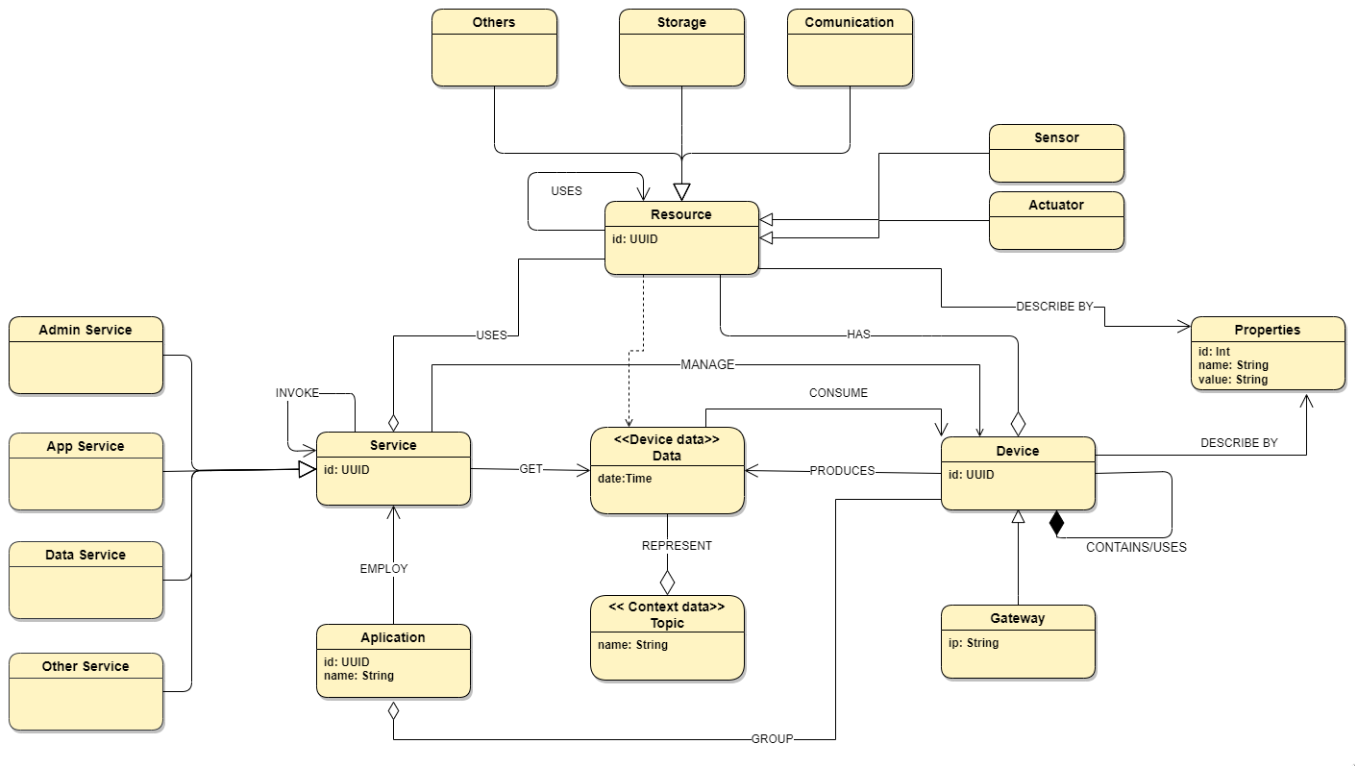
\includegraphics[width=\linewidth]{images/Henrymodelo.png}
\end{figure}

% En este modelo, se presentan todas los componentes que componen a Smart Campus UIS en términos de su arquitectura a un nivel técnico. Ahora, para modelar un Smart Campus a nivel de aplicación, se tomó una versión reducida de este modelo enfocándose en los componentes y a la función que estos cumplen en una ubicación geográfica dada. 

% El basarnos en este modelo nos asegura que se tiene la capacidad de realizar la descripción de un un sistema IoT de Smart Campus en un nivel técnico. Este contiene todos los componentes necesarios para poder modelar

Basarnos en el modelo de la figura \ref{fig:henrymodelo}, nos da la capacidad de describir a un nivel técnico un sistema IoT. Ahora, aunque se podría usar para el desarrollo del proyecto, fue necesario modificarlo con el fin de acercarnos más hacia la descripción de un sistema IoT a nivel de aplicación. 

Lo primero fue el establecer el contexto de los dispositivos. Esto específicamente se refiere al criterio \textit{C2} de la tabla \ref{tab:criterios}, en donde, dada la necesidad de establecer la ubicación geográfica en algunas de las aplicaciones de los Smart Campus, era necesario poder describir los lugares pertenecientes a la aplicación.

Así mismo, se cubre el criterio \textit{C3} cambiando las propiedades del dispositivos de una clase, externa a los dispositivos; a un atributo, interno, el cual le permite a los componentes manejar su propia información en cuanto a los datos que estos manejan. Estas propiedades puede referirse a las entradas que tienen, en el caso de ser actuadores o procesadores de la información; o a los valores que reportan al sistema en el caso de ser sensores.

Partiendo de esto, se planteó el modelo presente en la figura \ref{fig:metamodelo}.

\begin{figure}[H]
    \centering
    \caption{Versión 1 del metamodelo planteado para SCampusADL}
    \label{fig:metamodelo}
    \vspace{2mm}
    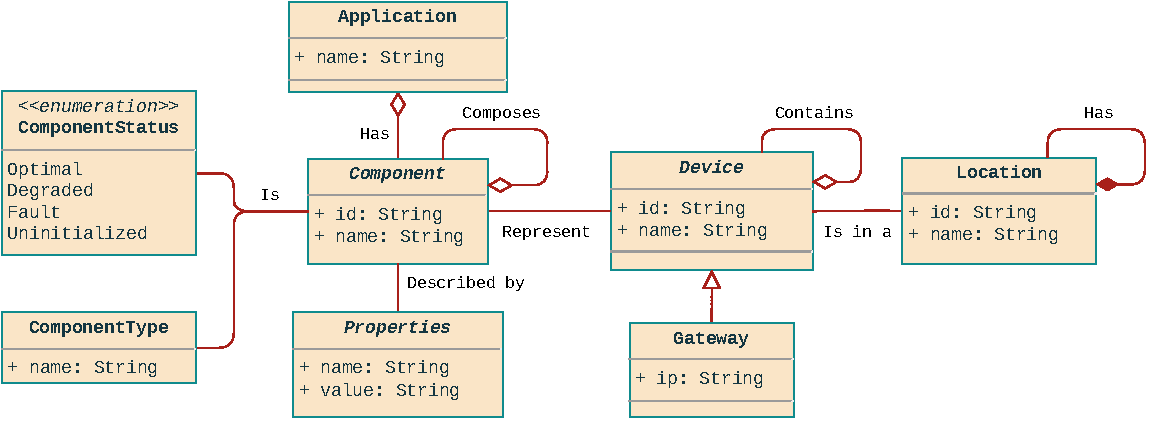
\includegraphics[width=\linewidth]{images/Metamodel.pdf}
\end{figure}

% Aquí seguiría la descripción del modelo presentado

% Y creo que después debería ir la definición de los estados de los dispositivos

% Y luego creo que iría la parte de la notación que es Yaml